\documentclass[]{article}
\usepackage{lmodern}
\usepackage{amssymb,amsmath}
\usepackage{ifxetex,ifluatex}
\usepackage{fixltx2e} % provides \textsubscript
\ifnum 0\ifxetex 1\fi\ifluatex 1\fi=0 % if pdftex
  \usepackage[T1]{fontenc}
  \usepackage[utf8]{inputenc}
\else % if luatex or xelatex
  \ifxetex
    \usepackage{mathspec}
  \else
    \usepackage{fontspec}
  \fi
  \defaultfontfeatures{Ligatures=TeX,Scale=MatchLowercase}
\fi
% use upquote if available, for straight quotes in verbatim environments
\IfFileExists{upquote.sty}{\usepackage{upquote}}{}
% use microtype if available
\IfFileExists{microtype.sty}{%
\usepackage{microtype}
\UseMicrotypeSet[protrusion]{basicmath} % disable protrusion for tt fonts
}{}
\usepackage[margin=1in]{geometry}
\usepackage{hyperref}
\hypersetup{unicode=true,
            pdftitle={Introducción al scraping y a la minería de texto},
            pdfauthor={Olivier Nuñez},
            pdfborder={0 0 0},
            breaklinks=true}
\urlstyle{same}  % don't use monospace font for urls
\usepackage{color}
\usepackage{fancyvrb}
\newcommand{\VerbBar}{|}
\newcommand{\VERB}{\Verb[commandchars=\\\{\}]}
\DefineVerbatimEnvironment{Highlighting}{Verbatim}{commandchars=\\\{\}}
% Add ',fontsize=\small' for more characters per line
\usepackage{framed}
\definecolor{shadecolor}{RGB}{248,248,248}
\newenvironment{Shaded}{\begin{snugshade}}{\end{snugshade}}
\newcommand{\KeywordTok}[1]{\textcolor[rgb]{0.13,0.29,0.53}{\textbf{#1}}}
\newcommand{\DataTypeTok}[1]{\textcolor[rgb]{0.13,0.29,0.53}{#1}}
\newcommand{\DecValTok}[1]{\textcolor[rgb]{0.00,0.00,0.81}{#1}}
\newcommand{\BaseNTok}[1]{\textcolor[rgb]{0.00,0.00,0.81}{#1}}
\newcommand{\FloatTok}[1]{\textcolor[rgb]{0.00,0.00,0.81}{#1}}
\newcommand{\ConstantTok}[1]{\textcolor[rgb]{0.00,0.00,0.00}{#1}}
\newcommand{\CharTok}[1]{\textcolor[rgb]{0.31,0.60,0.02}{#1}}
\newcommand{\SpecialCharTok}[1]{\textcolor[rgb]{0.00,0.00,0.00}{#1}}
\newcommand{\StringTok}[1]{\textcolor[rgb]{0.31,0.60,0.02}{#1}}
\newcommand{\VerbatimStringTok}[1]{\textcolor[rgb]{0.31,0.60,0.02}{#1}}
\newcommand{\SpecialStringTok}[1]{\textcolor[rgb]{0.31,0.60,0.02}{#1}}
\newcommand{\ImportTok}[1]{#1}
\newcommand{\CommentTok}[1]{\textcolor[rgb]{0.56,0.35,0.01}{\textit{#1}}}
\newcommand{\DocumentationTok}[1]{\textcolor[rgb]{0.56,0.35,0.01}{\textbf{\textit{#1}}}}
\newcommand{\AnnotationTok}[1]{\textcolor[rgb]{0.56,0.35,0.01}{\textbf{\textit{#1}}}}
\newcommand{\CommentVarTok}[1]{\textcolor[rgb]{0.56,0.35,0.01}{\textbf{\textit{#1}}}}
\newcommand{\OtherTok}[1]{\textcolor[rgb]{0.56,0.35,0.01}{#1}}
\newcommand{\FunctionTok}[1]{\textcolor[rgb]{0.00,0.00,0.00}{#1}}
\newcommand{\VariableTok}[1]{\textcolor[rgb]{0.00,0.00,0.00}{#1}}
\newcommand{\ControlFlowTok}[1]{\textcolor[rgb]{0.13,0.29,0.53}{\textbf{#1}}}
\newcommand{\OperatorTok}[1]{\textcolor[rgb]{0.81,0.36,0.00}{\textbf{#1}}}
\newcommand{\BuiltInTok}[1]{#1}
\newcommand{\ExtensionTok}[1]{#1}
\newcommand{\PreprocessorTok}[1]{\textcolor[rgb]{0.56,0.35,0.01}{\textit{#1}}}
\newcommand{\AttributeTok}[1]{\textcolor[rgb]{0.77,0.63,0.00}{#1}}
\newcommand{\RegionMarkerTok}[1]{#1}
\newcommand{\InformationTok}[1]{\textcolor[rgb]{0.56,0.35,0.01}{\textbf{\textit{#1}}}}
\newcommand{\WarningTok}[1]{\textcolor[rgb]{0.56,0.35,0.01}{\textbf{\textit{#1}}}}
\newcommand{\AlertTok}[1]{\textcolor[rgb]{0.94,0.16,0.16}{#1}}
\newcommand{\ErrorTok}[1]{\textcolor[rgb]{0.64,0.00,0.00}{\textbf{#1}}}
\newcommand{\NormalTok}[1]{#1}
\usepackage{longtable,booktabs}
\usepackage{graphicx,grffile}
\makeatletter
\def\maxwidth{\ifdim\Gin@nat@width>\linewidth\linewidth\else\Gin@nat@width\fi}
\def\maxheight{\ifdim\Gin@nat@height>\textheight\textheight\else\Gin@nat@height\fi}
\makeatother
% Scale images if necessary, so that they will not overflow the page
% margins by default, and it is still possible to overwrite the defaults
% using explicit options in \includegraphics[width, height, ...]{}
\setkeys{Gin}{width=\maxwidth,height=\maxheight,keepaspectratio}
\IfFileExists{parskip.sty}{%
\usepackage{parskip}
}{% else
\setlength{\parindent}{0pt}
\setlength{\parskip}{6pt plus 2pt minus 1pt}
}
\setlength{\emergencystretch}{3em}  % prevent overfull lines
\providecommand{\tightlist}{%
  \setlength{\itemsep}{0pt}\setlength{\parskip}{0pt}}
\setcounter{secnumdepth}{5}
% Redefines (sub)paragraphs to behave more like sections
\ifx\paragraph\undefined\else
\let\oldparagraph\paragraph
\renewcommand{\paragraph}[1]{\oldparagraph{#1}\mbox{}}
\fi
\ifx\subparagraph\undefined\else
\let\oldsubparagraph\subparagraph
\renewcommand{\subparagraph}[1]{\oldsubparagraph{#1}\mbox{}}
\fi

%%% Use protect on footnotes to avoid problems with footnotes in titles
\let\rmarkdownfootnote\footnote%
\def\footnote{\protect\rmarkdownfootnote}

%%% Change title format to be more compact
\usepackage{titling}

% Create subtitle command for use in maketitle
\newcommand{\subtitle}[1]{
  \posttitle{
    \begin{center}\large#1\end{center}
    }
}

\setlength{\droptitle}{-2em}
  \title{Introducción al scraping y a la minería de texto}
  \pretitle{\vspace{\droptitle}\centering\huge}
  \posttitle{\par}
  \author{Olivier Nuñez}
  \preauthor{\centering\large\emph}
  \postauthor{\par}
  \predate{\centering\large\emph}
  \postdate{\par}
  \date{2018-06-01}

\newenvironment{ej}{\begin{Shaded}}{\end{Shaded}}
\newenvironment{nota}{\begin{Shaded}}{\end{Shaded}}

\begin{document}
\maketitle

{
\setcounter{tocdepth}{2}
\tableofcontents
}
\section*{Preámbulo}\label{preambulo}
\addcontentsline{toc}{section}{Preámbulo}

Internet es una fuente inagotable de información y datos.
Desafortunadamente, la mayoría de las veces, los datos están integrados
a una pagina web y no pueden ser extraídos directamente para su análisis
estadístico.

Cuando el volumen de datos es pequeño, es posible copiarlos ``a mano''.
Pero si la cantidad de datos es demasiado grande o si están dispersos en
un gran número de páginas, este método no es factible.

Esta introducción tiene como objetivo explicar cómo extraer esta
información utilizando herramientas de R y mostrar algunas operaciones
de procesamiento y análisis de datos textuales.

Lo que sigue requiere los paquetes \texttt{rvest} y \texttt{tidytext}:

\begin{Shaded}
\begin{Highlighting}[]
\KeywordTok{install.packages}\NormalTok{(}\KeywordTok{c}\NormalTok{(}\StringTok{"rvest"}\NormalTok{,}\StringTok{"tidytext"}\NormalTok{),}\DataTypeTok{dep=}\OtherTok{TRUE}\NormalTok{)}
\end{Highlighting}
\end{Shaded}

\section{Scraping con R}\label{scraping-con-r}

\subsection{\texorpdfstring{Qué se puede ``rascar'' de la
web?}{Qué se puede rascar de la web?}}\label{que-se-puede-rascar-de-la-web}

\begin{quote}
``\emph{Si puedes verlo, puedes rascarlo}''
\end{quote}

Cualquier cosa en una página web:

\begin{itemize}
\tightlist
\item
  Tablas
\item
  Texto
\item
  Vínculos
\item
  Metadatos (tiempo de publicación, actualización, \ldots{})
\item
  Atributos de página web (colores, fuentes, tamaño de texto utilizado,
  ..)
\item
  Imágenes
\end{itemize}

\subsection{Formato HTML}\label{formato-html}

El código HTML está compuesto de etiquetas predefinidas que le dicen al
navegador cómo mostrar los datos. A menudo, estas etiquetas están
anidadas:

\begin{verbatim}
<ul>
    <li>Articulo 1</li>
    <li>Articulo 2</li>
</ul>
\end{verbatim}

Dará:

\begin{quote}
\begin{itemize}
\tightlist
\item
  Artículo 1
\item
  Artículo 2
\end{itemize}
\end{quote}

La etiqueta ``\textless{}ul\textgreater{}'' indica una lista desordenada
y ``\textless{}li\textgreater{}'' indica un elemento de la lista. Una
etiqueta que comienza con una barra inclinada finaliza la etiqueta
anterior de ese tipo.

HTML se vuelve más complicado, pero entender las etiquetas es suficiente
para comenzar a rascar.

\subsection{Identificar elementos de interés en una
página}\label{identificar-elementos-de-interes-en-una-pagina}

Puede ser útil ilustrar brevemente algunas prácticas para identificar
elementos en una página de la cual uno desea extraer los datos. En este
sentido, la mayoría de los navegadores web ofrecen no solo la
posibilidad de ver el código fuente de una página, sino también analizar
los elementos.

Esta función de \emph{inspección} suele estar disponible directamente en
el menú contextual del navegador. Se señala el elemento que nos
interesa, se hace clic con el botón derecho y se elige el elemento del
menú contextual que permite analizarlo.

Captura de pantalla de la pagina de IMDB dedicada a la película
``Amanece que no es poco'' 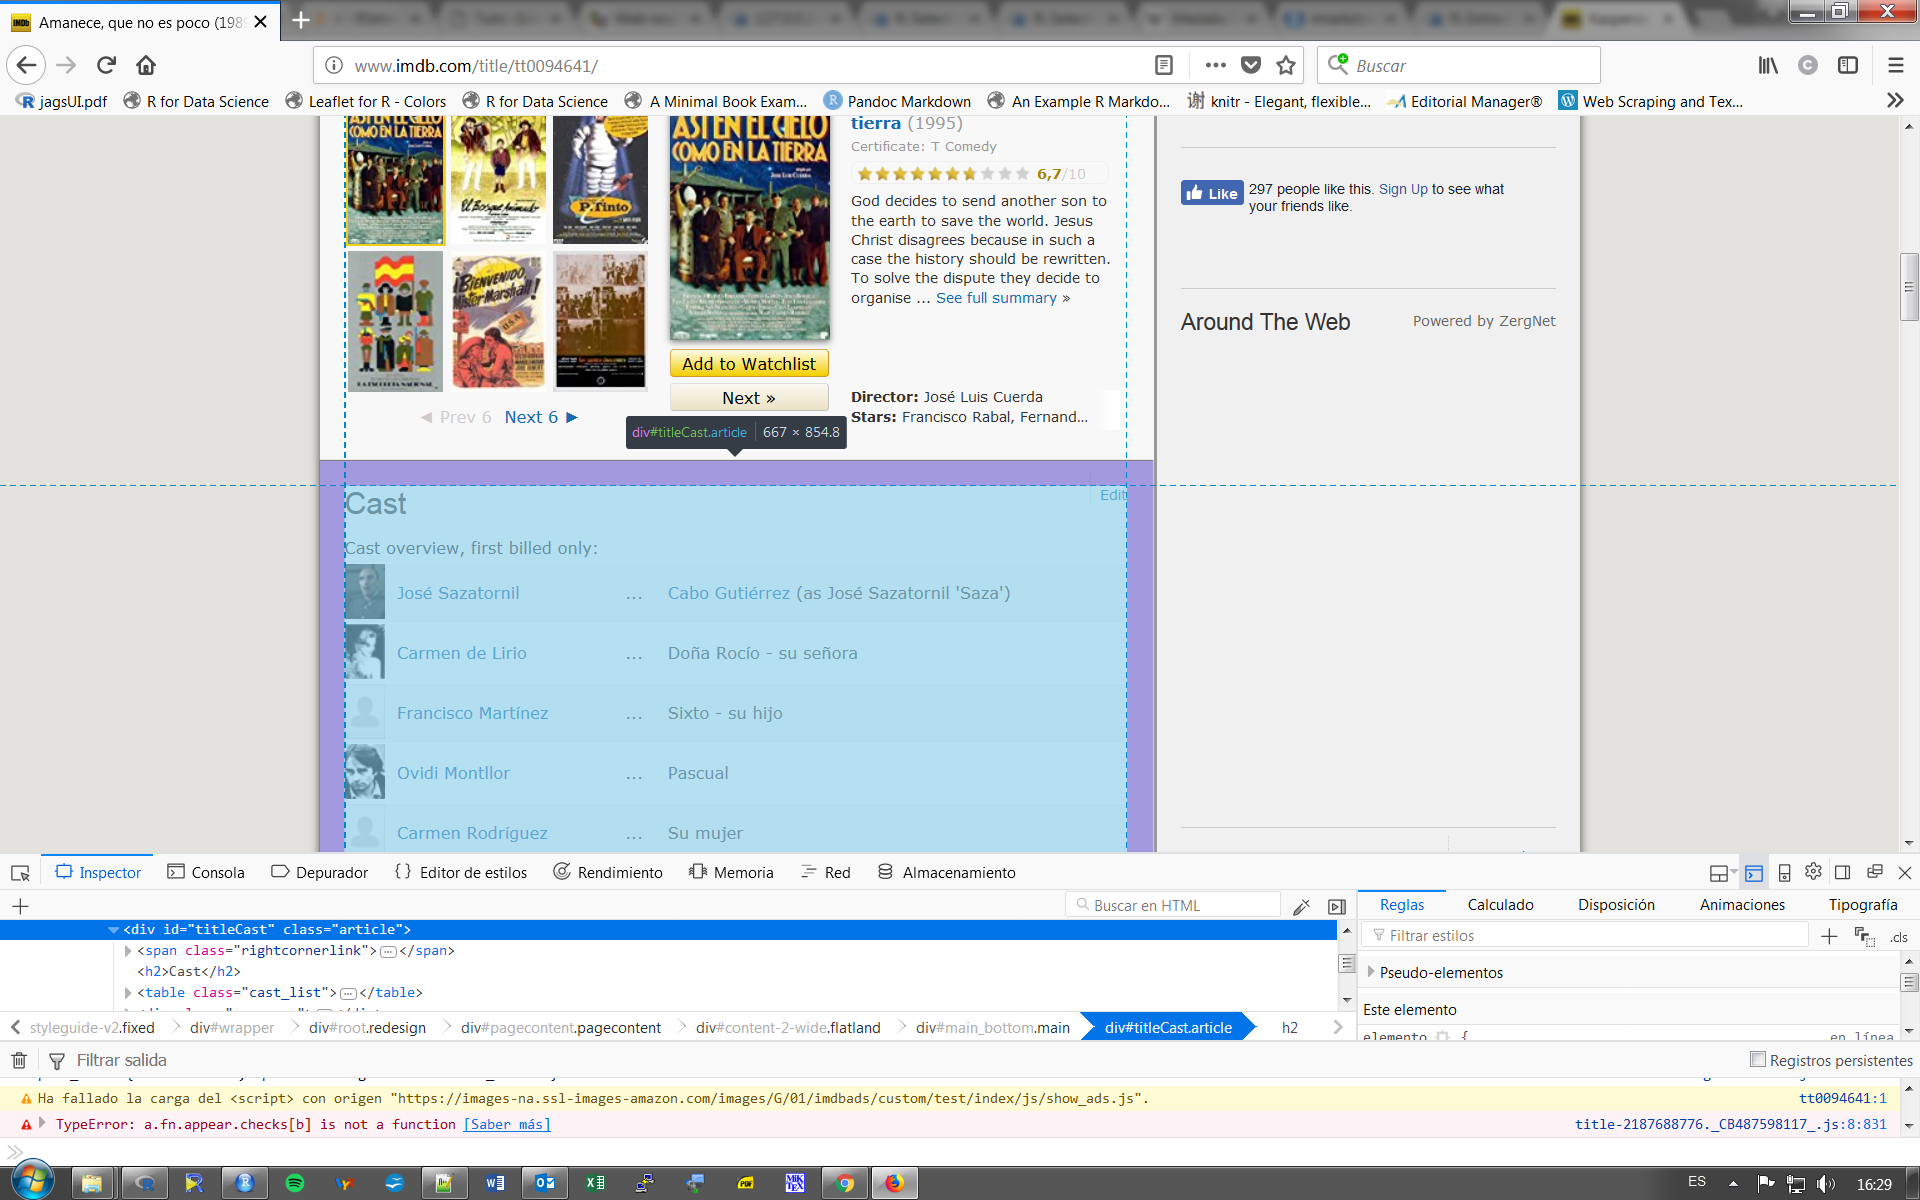
\includegraphics{images/amanece.png}

Aquí hay una lista de criterios para la identificación de los elementos:

\begin{itemize}
\item
  \textbf{ID} de atributo : si el elemento tiene un atributo id
  (caracterizado en el identificador con el carácter \#), se supone que
  este atributo es exclusivo del elemento. Por lo tanto, es muy útil
  para extraerlo de la página, pero no es adecuado para extraer
  elementos recursivos (por ejemplo, varios párrafos), ya que cada uno
  debe tener una identificación única.
\item
  \textbf{Clases} : Las clases son una buena forma de identificar
  elementos recursivos en el mismo nivel jerárquico. Por ejemplo, los
  comentarios de blog a menudo comparten la misma clase (por ejemplo,
  class = ``comment''). Para maximizar la probabilidad de identificar el
  elemento correcto, en el caso de que múltiples elementos en diferentes
  ubicaciones en la página tengan la misma clase, este criterio puede
  estar asociado con el nombre de la etiqueta (por ejemplo,
  div.comment).
\item
  \textbf{Posición jerárquica} : el análisis de elementos a menudo
  propone la posición relativa a la raíz del DOM ocupado por el elemento
  seleccionado. Se usa si las etiquetas nunca tienen atributos de
  identificación o clase.
\end{itemize}

\subsection{\texorpdfstring{El paquete
\texttt{rvest}}{El paquete rvest}}\label{el-paquete-rvest}

Este paquete de ``cosecha'' extrae contenidos de páginas web en HTML/XML
usando la sintaxis de los
\href{https://www.w3schools.com/cssref/css_selectors.asp}{selectores de
CSS}. Por ejemplo, un párrafo que está directamente dentro de una
etiqueta de tipo \emph{div} puede identificarse usando la notación
\emph{div \textgreater{} p}.

Este paquete es bastante simple, porque no tiene muchas funciones, pero
proporciona las principales características necesarias para la
identificación y extracción de datos en una página, así como algunas
funciones que permiten explorar las páginas emulando un navegador web.

\subsubsection{Cargar la pagina}\label{cargar-la-pagina}

Para ilustrar el uso de \texttt{rvest}, vamos a extraer información
sobre la película ``Amanece, que no es poco'' de su pagina en el
\href{http://www.imdb.com/title/tt0094641/}{IMDb}.

\begin{Shaded}
\begin{Highlighting}[]
\KeywordTok{require}\NormalTok{(rvest)}
\NormalTok{amanece <-}\StringTok{ }\KeywordTok{read_html}\NormalTok{(}\StringTok{"http://www.imdb.com/title/tt0094641/"}\NormalTok{)}
\end{Highlighting}
\end{Shaded}

La función \texttt{read\_html}permite importar en R el contenido html de
una página web. El argumento principal de esta función es la dirección
de la pagina web ( o el path de fichero html local).

\subsubsection{Extracción}\label{extraccion}

La función \texttt{html\_nodes} acepta dos argumentos, ambos necesarios:

\begin{verbatim}
html_nodes(x, css)
\end{verbatim}

\begin{itemize}
\tightlist
\item
  El argumento x representa el código HTML importado mediante la función
  \texttt{read\_html}
\item
  El segundo argumento es un criterio de selección que utiliza la
  gramática de los selectores de CSS.
\end{itemize}

Esta función devuelve una lista (matriz) de las ocurrencias encontradas
en la pagina de acuerdo al criterio de selección. Así, el comando
siguiente da la lista de las tablas incluidas en la pagina:

\begin{Shaded}
\begin{Highlighting}[]
\KeywordTok{html_nodes}\NormalTok{(amanece, }\StringTok{"table"}\NormalTok{) }
\end{Highlighting}
\end{Shaded}

\begin{verbatim}
## {xml_nodeset (2)}
## [1] <table class="cast_list">\n<tr><td colspan="4" class="castlist_label ...
## [2] <table class="footer" id="amazon-affiliates">\n<tr>\n<td colspan="8" ...
\end{verbatim}

\paragraph{Extracción de texto}\label{extraccion-de-texto}

Se puede también extraer su titulo

\begin{Shaded}
\begin{Highlighting}[]
\NormalTok{titulo <-}\StringTok{ }\KeywordTok{html_node}\NormalTok{(amanece, }\StringTok{"title"}\NormalTok{)}
\KeywordTok{html_text}\NormalTok{(titulo)}
\end{Highlighting}
\end{Shaded}

\begin{verbatim}
## [1] "Amanece, que no es poco (1989) - IMDb"
\end{verbatim}

Sólo hay una etiqueta ``title'' en una página, por lo que utilizaremos
\texttt{html\_node()} (sin la \emph{s} final) en lugar de
\texttt{html\_nodes()}, porque sólo devuelve un elemento en vez de una
lista.

La función \texttt{html\_text} elimina todas las etiquetas del código y
muestra solo el contenido textual. Una opción muy útil de esta función
es \texttt{trim\ =\ TRUE} que elimina los espacios antes y después del
texto.

Cabe mencionar, que mediante la gramática de ``tuberias'', la secuencia
anterior de comandos, puede ser expresada en una solo linea:

\begin{Shaded}
\begin{Highlighting}[]
\NormalTok{amanece }\OperatorTok\StringTok{ }\KeywordTok{html_node}\NormalTok{(}\StringTok{"title"}\NormalTok{) }\OperatorTok\StringTok{ }\KeywordTok{html_text}\NormalTok{()}
\end{Highlighting}
\end{Shaded}

\begin{ej}
Descargar el ultimo discurso del rey de España desde la siguiente
dirección:

\url{http://www.casareal.es/ES/Actividades/Paginas/actividades_discursos_detalle.aspx?data=5738}
\end{ej}

\paragraph{Extracción de tablas}\label{extraccion-de-tablas}

La función \texttt{html\_table}, como su nombre indica, está
especialmente diseñada para extraer los contenidos de una tabla HTML,
manteniendo la estructura en filas y columnas-

Así, el comando siguiente permite extraer la lista de actores de la
película que viene en la segunda columna de la tabla con clase
``cast\_list'':

\begin{Shaded}
\begin{Highlighting}[]
\KeywordTok{html_node}\NormalTok{(amanece, }\StringTok{"table.cast_list"}\NormalTok{) }\OperatorTok\StringTok{ }\KeywordTok{html_table}\NormalTok{(}\DataTypeTok{header=}\OtherTok{TRUE}\NormalTok{) }\OperatorTok\StringTok{ }\NormalTok{.[[}\DecValTok{2}\NormalTok{]] }\CommentTok{# .[[2]] para segunda columna}
\end{Highlighting}
\end{Shaded}

\begin{verbatim}
##  [1] "José Sazatornil"     "Carmen de Lirio"     "Francisco Martínez" 
##  [4] "Ovidi Montllor"      "Carmen Rodríguez"    "Rafael Díaz"        
##  [7] "Amada Tercero"       "Cassen"              "Manuel Alexandre"   
## [10] "María Ángeles Ariza" "Rafael Alonso"       "Fedra Lorente"      
## [13] "Cris Huerta"         "Elisa Belmonte"      "María I. González"
\end{verbatim}

\begin{ej}
Descargar las cotizaciones del IBEX 35 en tiempo real desde la siguiente
pagina

ibex35 \textless{}-
``\url{http://www.bolsamadrid.es/esp/aspx/Mercados/Precios.aspx?indice=ESI100000000}''
\end{ej}

\paragraph{Extracción de vinculos}\label{extraccion-de-vinculos}

Para ilustrar este tipo de extracción, vamos a importar las direcciones
de las paginas de los actores de la película. Empezamos importando todos
los enlaces (etiqueta `\textless{}a\textgreater{}´de ``ancla'')
contenidos en una tabla:

\begin{Shaded}
\begin{Highlighting}[]
\NormalTok{enlaces <-}\StringTok{ }\KeywordTok{html_nodes}\NormalTok{(amanece, }\StringTok{"table a"}\NormalTok{)}
\NormalTok{enlaces}
\end{Highlighting}
\end{Shaded}

\begin{verbatim}
## {xml_nodeset (41)}
##  [1] <a href="/name/nm0768574/?ref_=tt_cl_i1"><img height="44" width="32 ...
##  [2] <a href="/name/nm0768574/?ref_=tt_cl_t1" itemprop="url"> <span clas ...
##  [3] <a href="/title/tt0094641/characters/nm0768574?ref_=tt_cl_t1">Cabo  ...
##  [4] <a href="/name/nm0513922/?ref_=tt_cl_i2"><img height="44" width="32 ...
##  [5] <a href="/name/nm0513922/?ref_=tt_cl_t2" itemprop="url"> <span clas ...
##  [6] <a href="/name/nm1771790/?ref_=tt_cl_i3"><img height="44" width="32 ...
##  [7] <a href="/name/nm1771790/?ref_=tt_cl_t3" itemprop="url"> <span clas ...
##  [8] <a href="/name/nm0600120/?ref_=tt_cl_i4"><img height="44" width="32 ...
##  [9] <a href="/name/nm0600120/?ref_=tt_cl_t4" itemprop="url"> <span clas ...
## [10] <a href="/name/nm1771909/?ref_=tt_cl_i5"><img height="44" width="32 ...
## [11] <a href="/name/nm1771909/?ref_=tt_cl_t5" itemprop="url"> <span clas ...
## [12] <a href="/name/nm0246717/?ref_=tt_cl_i6"><img height="44" width="32 ...
## [13] <a href="/name/nm0246717/?ref_=tt_cl_t6" itemprop="url"> <span clas ...
## [14] <a href="/name/nm1773519/?ref_=tt_cl_i7"><img height="44" width="32 ...
## [15] <a href="/name/nm1773519/?ref_=tt_cl_t7" itemprop="url"> <span clas ...
## [16] <a href="/name/nm0144107/?ref_=tt_cl_i8"><img height="44" width="32 ...
## [17] <a href="/name/nm0144107/?ref_=tt_cl_t8" itemprop="url"> <span clas ...
## [18] <a href="/title/tt0094641/characters/nm0144107?ref_=tt_cl_t8">Cura  ...
## [19] <a href="/name/nm0018872/?ref_=tt_cl_i9"><img height="44" width="32 ...
## [20] <a href="/name/nm0018872/?ref_=tt_cl_t9" itemprop="url"> <span clas ...
## ...
\end{verbatim}

Luego extraemos las direcciones (atributo \texttt{href}) a las que
apuntan dichos enlaces utilizando la función \texttt{html\_attr}:

\begin{Shaded}
\begin{Highlighting}[]
\NormalTok{actores <-}\StringTok{ }\NormalTok{enlaces }\OperatorTok\StringTok{ }\KeywordTok{html_attr}\NormalTok{(}\StringTok{"href"}\NormalTok{)}
\NormalTok{raiz=}\StringTok{"http://www.imdb.com"}
\KeywordTok{browseURL}\NormalTok{(}\KeywordTok{paste}\NormalTok{(raiz,actores[}\DecValTok{1}\NormalTok{],}\DataTypeTok{sep=}\StringTok{"/"}\NormalTok{)) }\CommentTok{#pagina de José Sazatornil }
\end{Highlighting}
\end{Shaded}

\subsection{Navegación}\label{navegacion}

El paquete \texttt{rvest} proporciona también funciones para emular un
navegador web.

\subsubsection{Inición de la navegación}\label{inicion-de-la-navegacion}

Con la función \texttt{html\_session}se crea un punto de entrada para la
navegación.

\begin{Shaded}
\begin{Highlighting}[]
\NormalTok{sesion <-}\StringTok{ }\KeywordTok{html_session}\NormalTok{(}\StringTok{"http://www.imdb.com"}\NormalTok{)}
\end{Highlighting}
\end{Shaded}

La variable ``sesion'' contiene ahora información de la página
``visitada''.

\begin{Shaded}
\begin{Highlighting}[]
\NormalTok{sesion }
\end{Highlighting}
\end{Shaded}

\begin{verbatim}
## <session> https://www.imdb.com/
##   Status: 200
##   Type:   text/html;charset=UTF-8
##   Size:   192658
\end{verbatim}

\subsubsection{\texorpdfstring{Funciones \texttt{jump\_to} y
\texttt{follow\_link}}{Funciones jump\_to y follow\_link}}\label{funciones-jump_to-y-follow_link}

Estas dos funciones tienen el mismo propósito, es decir, seguir un
enlace para ir de una página a otra. La diferencia entre las dos
funciones se refiere a la forma de referirse al enlace.

La función \texttt{jump\_to} toma una url (ya sea relativa o absoluta)

\begin{Shaded}
\begin{Highlighting}[]
\NormalTok{sesion }\OperatorTok\StringTok{  }\KeywordTok{jump_to}\NormalTok{(}\StringTok{"boxoffice"}\NormalTok{) }\OperatorTok\StringTok{ }\KeywordTok{session_history}\NormalTok{()}
\end{Highlighting}
\end{Shaded}

\begin{verbatim}
##   https://www.imdb.com/
## - https://www.imdb.com/chart/boxoffice
\end{verbatim}

Mientras que la función \texttt{follow\_link} acepta la referencia a un
enlace en una página en tres formas distintas:

\begin{itemize}
\tightlist
\item
  Un número cardinal (ej., ``5'' para la quinta etiqueta \texttt{a}
  presente en el HTML de la página).
\item
  Un selector CSS (ej., ``p a'' para enlaces en un párrafo)
\item
  Una palabra o frase que representa la etiqueta textual del enlace (ej.
  )
\end{itemize}

toma una expresión que hace referencia a un enlace (una etiqueta
\emph{\textless{}a\textgreater{}}) de la página:

\begin{Shaded}
\begin{Highlighting}[]
\NormalTok{sesion }\OperatorTok\StringTok{ }\KeywordTok{follow_link}\NormalTok{(}\DecValTok{5}\NormalTok{)}
\end{Highlighting}
\end{Shaded}

\begin{verbatim}
## Navigating to /chart/toptv/?ref_=nv_tp_tv250_2
\end{verbatim}

\begin{verbatim}
## <session> https://www.imdb.com/chart/toptv/?ref_=nv_tp_tv250_2
##   Status: 200
##   Type:   text/html;charset=UTF-8
##   Size:   572853
\end{verbatim}

\begin{Shaded}
\begin{Highlighting}[]
\NormalTok{sesion }\OperatorTok\StringTok{ }\KeywordTok{follow_link}\NormalTok{(}\DataTypeTok{css =} \StringTok{"p a"}\NormalTok{) }\CommentTok{#enlace en un parráfo}
\end{Highlighting}
\end{Shaded}

\begin{verbatim}
## Navigating to /movies-in-theaters/?ref_=nv_tp_inth_1
\end{verbatim}

\begin{verbatim}
## <session> https://www.imdb.com/movies-in-theaters/?ref_=nv_tp_inth_1
##   Status: 200
##   Type:   text/html;charset=UTF-8
##   Size:   198241
\end{verbatim}

\begin{Shaded}
\begin{Highlighting}[]
\NormalTok{sesion }\OperatorTok\StringTok{ }\KeywordTok{follow_link}\NormalTok{(}\StringTok{"Indian"}\NormalTok{)}
\end{Highlighting}
\end{Shaded}

\begin{verbatim}
## Navigating to /india/top-rated-indian-movies?ref_=nv_mv_250_in_7
\end{verbatim}

\begin{verbatim}
## <session> https://www.imdb.com/india/top-rated-indian-movies/?ref_=nv_mv_250_in_7
##   Status: 200
##   Type:   text/html;charset=UTF-8
##   Size:   592337
\end{verbatim}

Cualquier movimiento con estas funciones se grabará en la sesión de
navegación, de modo que se pueda realizar un seguimiento de la
navegación. La función \texttt{session\_history} muestra la cronología
completa de las páginas visitadas en la misma sesión:

\begin{Shaded}
\begin{Highlighting}[]
\NormalTok{sesion }\OperatorTok\StringTok{  }\KeywordTok{jump_to}\NormalTok{(}\StringTok{"boxoffice"}\NormalTok{) }\OperatorTok\StringTok{ }\KeywordTok{session_history}\NormalTok{()}
\end{Highlighting}
\end{Shaded}

\begin{verbatim}
##   https://www.imdb.com/
## - https://www.imdb.com/chart/boxoffice
\end{verbatim}

\subsubsection{html\_form(sesion)}\label{html_formsesion}

\begin{Shaded}
\begin{Highlighting}[]
\KeywordTok{html_form}\NormalTok{(sesion)}
\end{Highlighting}
\end{Shaded}

\begin{verbatim}
## [[1]]
## <form> 'navbar-form' (GET /find)
##   <button submit> '<unnamed>
##   <input hidden> 'ref_': nv_sr_fn
##   <input text> 'q': 
##   <select> 's' [0/6]
## 
## [[2]]
## <form> 'ue_backdetect' (GET get)
##   <input hidden> 'ue_back': 1
\end{verbatim}

Buscamos las películas con ``amanece'' en su título:

\begin{Shaded}
\begin{Highlighting}[]
\NormalTok{busqueda <-}\KeywordTok{html_form}\NormalTok{(sesion)[[}\DecValTok{1}\NormalTok{]] }\OperatorTok\StringTok{ }\KeywordTok{set_values}\NormalTok{(}\StringTok{`}\DataTypeTok{q}\StringTok{`}\NormalTok{ =}\StringTok{ "amanece"}\NormalTok{, }\DataTypeTok{s=}\StringTok{"Titles"}\NormalTok{) }
\NormalTok{busqueda }\OperatorTok\StringTok{ }\KeywordTok{submit_form}\NormalTok{(}\DataTypeTok{session=}\NormalTok{sesion) }\OperatorTok\StringTok{ }\KeywordTok{html_nodes}\NormalTok{(}\StringTok{"td.result_text"}\NormalTok{) }\OperatorTok\StringTok{ }\KeywordTok{html_text}\NormalTok{()}
\end{Highlighting}
\end{Shaded}

\begin{verbatim}
## Submitting with '<unnamed>'
\end{verbatim}

\begin{verbatim}
##  [1] " Le jour se lève (1939) aka \"Amanece\" "       
##  [2] " Amanece (2017) (Short) "                       
##  [3] " Amanece (2010) (Short) "                       
##  [4] " La saga Crepúsculo: Amanecer - Parte 2 (2012) "
##  [5] " Amanda Jane Cooper (Actress, Selfie (2014))"   
##  [6] " Dan Eckman (Director, Checkout (2006))"        
##  [7] " breaking-a-man's-neck (4 titles) "             
##  [8] " andaman-sea (2 titles) "                       
##  [9] " Amanecer Latino [es] (Production) "            
## [10] " Amanecer Films [es] (Production) "
\end{verbatim}

\begin{ej}
Extraer cotizaciones del ibex 35 utilizando navegación virtual. Inicio
de sesión:

cotiz \textless{}-
html\_session(``\url{http://www.bolsamadrid.es/esp/aspx/Mercados/Precios.aspx}'')
\end{ej}

\section{Introducción a la minería de
texto}\label{introduccion-a-la-mineria-de-texto}

\subsection{Aplicaciones}\label{aplicaciones}

La minería de texto nace de una combinación de minería de datos,
análisis de texto cuantitativo y procesamiento automático del lenguaje.

Las principales aplicaciones son:

\begin{itemize}
\tightlist
\item
  Motores de búsqueda
\item
  Detección de plagio
\item
  Clasificación de correo electrónico (detección de SPAM)
\item
  Búsqueda de opiniones (evaluaciones positivas o negativas de un
  servicio, etc.)
\item
  Organización de información (tipologías, ontologías)
\item
  Traducción automática
\item
  \ldots{}
\end{itemize}

\subsection{Conceptos básicos}\label{conceptos-basicos}

\subsubsection{Formato de los datos
textuales}\label{formato-de-los-datos-textuales}

Podemos distinguir tres tipos principales de textos:

\begin{enumerate}
\def\labelenumi{\arabic{enumi}.}
\tightlist
\item
  Tablas que consisten en filas y columnas
\item
  Textos sin formato (extracción de pdf, \ldots{})
\item
  Documentos semiestructurados (paginas web, correos electrónicos, RSS)
\end{enumerate}

\subsubsection{Unidad de análisis: el
token}\label{unidad-de-analisis-el-token}

Un \textbf{token} es una unidad significativa de texto, a menudo una
palabra (o una secuencia de palabras, oración, ..), en la cual estamos
interesados en utilizar para un análisis posterior. La
\textbf{tokenización} es el proceso de dividir el texto en tokens y es
uno de los primeros pasos del análisis de textos.

\subsubsection{Preparación de los datos
textuales}\label{preparacion-de-los-datos-textuales}

Antes de poder utilizar métodos puramente cuantitativos de minería de
textos, se debe preparar los documentos. Como regla general, pasamos por
los siguientes pasos (no necesariamente en este orden preciso):

\begin{enumerate}
\def\labelenumi{\arabic{enumi}.}
\tightlist
\item
  Creación del corpus
\item
  Limpieza y filtraje de la información relevante
\item
  Análisis del texto e interpretación de los resultados
\end{enumerate}

\subsection{Manipulación y análisis básicos de
texto}\label{manipulacion-y-analisis-basicos-de-texto}

Las tablas bajadas de Internet (y datos procedentes de otras fuentes)
exigen frecuentemente un proceso de limpieza de datos o de extracción de
la información que contienen.

La función \texttt{gsub} se usa muy a menudo para dicha limpieza de
datos. Una llamada a \texttt{gsub} tiene la forma

\begin{Shaded}
\begin{Highlighting}[]
\KeywordTok{gsub}\NormalTok{(}\StringTok{"h"}\NormalTok{, }\StringTok{"H"}\NormalTok{, }\KeywordTok{c}\NormalTok{(}\StringTok{"hola"}\NormalTok{, }\StringTok{"búho"))}
\end{Highlighting}
\end{Shaded}

\begin{verbatim}
## [1] "Hola" "búHo"
\end{verbatim}

donde el primer argumento, \texttt{"h"} es una
\href{https://es.wikipedia.org/wiki/Expresi\%C3\%B3n_regular}{expresión
regular}; la función \texttt{gsub} modifica las ocurrencias de esta
expresión regular por el segundo argumento, \texttt{"H"} en este caso.
El tercer argumento es un vector que contiene cadenas de texto en las
que se realiza la sustitución.

Las expresiones regulares son muy útiles para manipular texto. Conviene
aprender algunas de las más frecuentes, como por ejemplo, las que
identifican caracteres que aparecen al principio de un texto,

\begin{Shaded}
\begin{Highlighting}[]
\KeywordTok{gsub}\NormalTok{(}\StringTok{"^h"}\NormalTok{, }\StringTok{"H"}\NormalTok{, }\KeywordTok{c}\NormalTok{(}\StringTok{"hola"}\NormalTok{, }\StringTok{"búho"))}
\end{Highlighting}
\end{Shaded}

\begin{verbatim}
## [1] "Hola" "búho"
\end{verbatim}

o al final del mismo,

\begin{Shaded}
\begin{Highlighting}[]
\KeywordTok{gsub}\NormalTok{(}\StringTok{"o$"}\NormalTok{, }\StringTok{"os"}\NormalTok{, }\KeywordTok{c}\NormalTok{(}\StringTok{"hola"}\NormalTok{, }\StringTok{"búho"))}
\end{Highlighting}
\end{Shaded}

\begin{verbatim}
## [1] "hola"  "búhos"
\end{verbatim}

Una función emparentada con \texttt{gsub} es \texttt{grep}, que busca
cadenas en las que aparece una determinada expresión regular:

\begin{Shaded}
\begin{Highlighting}[]
\KeywordTok{grep}\NormalTok{(}\StringTok{"^h"}\NormalTok{, }\KeywordTok{c}\NormalTok{(}\StringTok{"hola"}\NormalTok{, }\StringTok{"búho"))}
\end{Highlighting}
\end{Shaded}

\begin{verbatim}
## [1] 1
\end{verbatim}

La salida de la expresión anterior nos indica que el patrón \emph{cadena
de texto que comienza con la letra h} aparece solo en la posición número
1 del vector.

\begin{ej}
\texttt{colors()} es una función que devuelve el nombre de más de 600
colores en R. Usándolo,

Encontrar * Aquellos cuyo nombre contenga un número (posiblemente tengas
que investigar cómo se expresa \emph{cualquier número} como expresión
regular) * Aquellos que comiencen con \texttt{yellow} * Aquellos que
contengan \texttt{blue}
\end{ej}

\begin{ej}
Los números que aparecen en la tabla descargada en la sección anterior
(y contenidos en \texttt{ibex}) no tienen formato numérico. Para
convertirlos en números \emph{de verdad}, transfórmalos adecuadamente:

\begin{itemize}
\tightlist
\item
  Usar \texttt{gsub} para cambiar ``.'' por ``'' (i.e., nada) en las
  columnas de interés. Ten en cuenta que \texttt{.} es el comodín de las
  expresiones regulares; el punto es
  \texttt{\textbackslash{}\textbackslash{}.}.
\item
  Usar \texttt{gsub} para cambiar \texttt{,} por \texttt{.} en las
  columnas de interés.
\item
  Finalmente, usar \texttt{as.numeric} para cambiar texto resultante por
  valores numéricos.
\end{itemize}
\end{ej}

Otra función muy útil para procesar texto es \texttt{paste}, que tiene
un comportamiento distinto según se use con el argumento \texttt{sep} o
\texttt{collapse}.

\begin{Shaded}
\begin{Highlighting}[]
\KeywordTok{paste}\NormalTok{(}\StringTok{"A"}\NormalTok{, }\DecValTok{1}\OperatorTok{:}\DecValTok{6}\NormalTok{, }\DataTypeTok{sep =} \StringTok{","}\NormalTok{)}
\end{Highlighting}
\end{Shaded}

\begin{verbatim}
## [1] "A,1" "A,2" "A,3" "A,4" "A,5" "A,6"
\end{verbatim}

\begin{Shaded}
\begin{Highlighting}[]
\KeywordTok{paste}\NormalTok{(}\StringTok{"Hoy es "}\NormalTok{, }\KeywordTok{date}\NormalTok{(), }\StringTok{" y tengo clase de R"}\NormalTok{, }\DataTypeTok{sep =} \StringTok{""}\NormalTok{)}
\end{Highlighting}
\end{Shaded}

\begin{verbatim}
## [1] "Hoy es Fri Jun 01 10:11:42 2018 y tengo clase de R"
\end{verbatim}

\begin{Shaded}
\begin{Highlighting}[]
\KeywordTok{paste}\NormalTok{(}\StringTok{"A"}\NormalTok{, }\DecValTok{1}\OperatorTok{:}\DecValTok{6}\NormalTok{, }\DataTypeTok{collapse =} \StringTok{","}\NormalTok{)}
\end{Highlighting}
\end{Shaded}

\begin{verbatim}
## [1] "A 1,A 2,A 3,A 4,A 5,A 6"
\end{verbatim}

\texttt{sep} y \texttt{collapse} pueden combinarse:

\begin{Shaded}
\begin{Highlighting}[]
\KeywordTok{paste}\NormalTok{(}\StringTok{"A"}\NormalTok{, }\DecValTok{1}\OperatorTok{:}\DecValTok{6}\NormalTok{, }\DataTypeTok{sep =} \StringTok{"_"}\NormalTok{, }\DataTypeTok{collapse =} \StringTok{","}\NormalTok{)}
\end{Highlighting}
\end{Shaded}

\begin{verbatim}
## [1] "A_1,A_2,A_3,A_4,A_5,A_6"
\end{verbatim}

Para la operación inversa, la de partir cadenas de texto, se usa la
función \texttt{strsplit}:

\begin{Shaded}
\begin{Highlighting}[]
\KeywordTok{strsplit}\NormalTok{(}\StringTok{"Hoy es martes"}\NormalTok{, }\DataTypeTok{split =} \StringTok{" "}\NormalTok{)}
\end{Highlighting}
\end{Shaded}

\begin{verbatim}
## [[1]]
## [1] "Hoy"    "es"     "martes"
\end{verbatim}

\begin{Shaded}
\begin{Highlighting}[]
\KeywordTok{strsplit}\NormalTok{(}\KeywordTok{c}\NormalTok{(}\StringTok{"hoy es martes"}\NormalTok{, }\StringTok{"mañana es miércoles"}\NormalTok{), }\DataTypeTok{split =} \StringTok{" "}\NormalTok{)}
\end{Highlighting}
\end{Shaded}

\begin{verbatim}
## [[1]]
## [1] "hoy"    "es"     "martes"
## 
## [[2]]
## [1] "mañana"    "es"        "miércoles"
\end{verbatim}

Advierte que esta función devuelve una lista de cadenas de texto.

\begin{ej}
Crea una función que tome los nombres de ficheros

\texttt{ficheros\ \textless{}-\ c("ventas\_20160522\_zaragoza.csv",\ \ \ \ \ \ \ \ \ \ \ \ \ \ \ \ \ "pedidos\_firmes\_20160422\_soria.csv")}

y genere una tabla con una fila por fichero y tres columnas: el nombre
del fichero, la fecha y y la provincia. Nota: puedes crear una función
que procese solo un nombre de fichero y aplicársela
\emph{convenientemente} al vector de nombres.
\end{ej}

Esas son las funciones fundamentales para la manipulación básica de
texto en R. Existen funciones más ágiles en otros paquetes como
\texttt{stringr}o \texttt{tidyr}.

A continuación una aplicación de uso del paquete \texttt{stringr} donde
se describe como se distribuyen las Medallas Fields (el ``nobel'' en
matemáticas) entre los países, utilizando la información proporcionada
por la wikipedia.

Empezamos extrayendo la tabla de interés desde la Wikipedia:

\begin{Shaded}
\begin{Highlighting}[]
\KeywordTok{require}\NormalTok{(rvest)}
\NormalTok{mfield<-}\KeywordTok{read_html}\NormalTok{(}\StringTok{"https://es.wikipedia.org/w/index.php?title=Medalla_Fields&oldid=103644843"}\NormalTok{)}
\NormalTok{mfield }\OperatorTok\StringTok{ }\KeywordTok{html_nodes}\NormalTok{(}\StringTok{"table"}\NormalTok{) }
\end{Highlighting}
\end{Shaded}

\begin{verbatim}
## {xml_nodeset (2)}
## [1] <table class="infobox" style="width:22.7em; line-height: 1.4em; text ...
## [2] <table class="wikitable" border="1">\n<tr>\n<th>Año</th>\n<th>Medall ...
\end{verbatim}

\begin{Shaded}
\begin{Highlighting}[]
\NormalTok{tabla <-}\StringTok{ }\NormalTok{mfield }\OperatorTok\StringTok{ }\KeywordTok{html_nodes}\NormalTok{(}\StringTok{"table"}\NormalTok{) }\OperatorTok\StringTok{ }\NormalTok{.[[}\DecValTok{2}\NormalTok{]] }\OperatorTok\StringTok{ }\KeywordTok{html_table}\NormalTok{(}\DataTypeTok{header=}\OtherTok{TRUE}\NormalTok{)}
\NormalTok{knitr}\OperatorTok{:::}\KeywordTok{kable}\NormalTok{(tabla }\OperatorTok\StringTok{ }\KeywordTok{head}\NormalTok{(}\DecValTok{10}\NormalTok{))}
\end{Highlighting}
\end{Shaded}

\begin{tabular}{r|l}
\hline
Año & Medallistas\\
\hline
1936 & Lars Ahlfors ( Finlandia), Universidad Harvard\\
\hline
1936 & Jesse Douglas ( Estados Unidos), Instituto Tecnológico de Massachusetts\\
\hline
1950 & Laurent Schwartz ( Francia), Universidad de Nancy\\
\hline
1950 & Atle Selberg (Noruega), Instituto de Estudios Avanzados de Princeton\\
\hline
1954 & Kunihiko Kodaira ( Japón), Universidad de Princeton\\
\hline
1954 & Jean-Pierre Serre ( Francia), Universidad de París\\
\hline
1958 & Klaus Friedrich Roth ( Reino Unido), Universidad de Londres\\
\hline
1958 & René Thom ( Francia), Universidad de Estrasburgo\\
\hline
1962 & Lars V. Hörmander (Suecia), Universidad de Estocolmo\\
\hline
1962 & John Willard Milnor ( Estados Unidos), Universidad de Princeton\\
\hline
\end{tabular}

Ahora, se extraen los países que vienen entre paréntesis usando
expresiones regulares
(\href{https://stat.ethz.ch/R-manual/R-devel/library/base/html/regex.html\%20(ayuda\%20de\%20R)}{ver
ayuda de R sobre estas expresiones}:

\begin{Shaded}
\begin{Highlighting}[]
\KeywordTok{require}\NormalTok{(tidyverse)}
\NormalTok{tmp <-}\StringTok{ }\NormalTok{tabla}\OperatorTok{$}\NormalTok{Medallistas }\OperatorTok\StringTok{ }\KeywordTok{str_extract}\NormalTok{(}\StringTok{"}\CharTok{\textbackslash{}\textbackslash{}}\StringTok{([^()]+}\CharTok{\textbackslash{}\textbackslash{}}\StringTok{)"}\NormalTok{) }\CommentTok{#extrae contenido entre parentesis }
\NormalTok{tmp <-}\StringTok{ }\KeywordTok{substring}\NormalTok{(tmp,}\DecValTok{2}\NormalTok{,}\KeywordTok{nchar}\NormalTok{(tmp)}\OperatorTok{-}\DecValTok{1}\NormalTok{)}
\NormalTok{paises<-}\StringTok{ }\NormalTok{tmp }\OperatorTok\StringTok{ }\KeywordTok{str_split_fixed}\NormalTok{(}\StringTok{" y "}\NormalTok{, }\DecValTok{2}\NormalTok{) }\OperatorTok\StringTok{ }\KeywordTok{str_trim}\NormalTok{() }\OperatorTok\StringTok{ }\KeywordTok{c}\NormalTok{()}
\end{Highlighting}
\end{Shaded}

Representación de distribución de medallas entre los países:

\begin{Shaded}
\begin{Highlighting}[]
\NormalTok{freq=}\KeywordTok{c}\NormalTok{(}\KeywordTok{table}\NormalTok{(paises))[}\OperatorTok{-}\DecValTok{1}\NormalTok{] }\CommentTok{#el -1 es para quitar la frecuencia de ""}
\KeywordTok{qplot}\NormalTok{(freq,}\KeywordTok{reorder}\NormalTok{(}\KeywordTok{names}\NormalTok{(freq),freq),}\DataTypeTok{ylab=}\StringTok{"paises"}\NormalTok{)}
\end{Highlighting}
\end{Shaded}

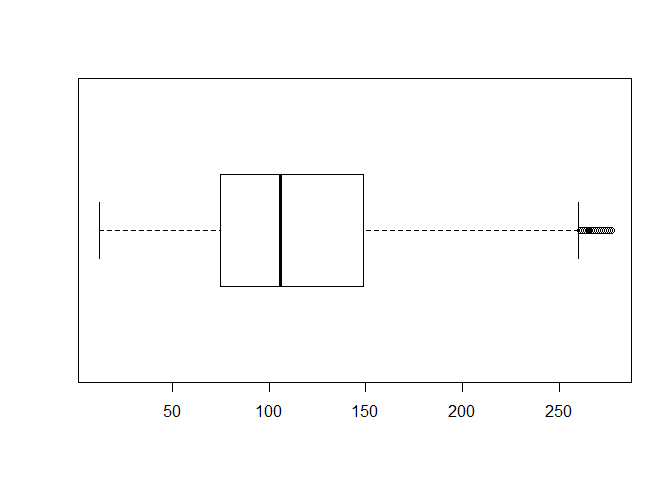
\includegraphics{IntroTextMining_files/figure-latex/unnamed-chunk-31-1.pdf}

\subsection{\texorpdfstring{Creación de un Corpus con
\texttt{tidytext}}{Creación de un Corpus con tidytext}}\label{creacion-de-un-corpus-con-tidytext}

El formato de texto \texttt{tidy} es básicamente una tabla con un
\textbf{token} por fila. Este formato se presta muy bien a la minería de
datos textuales.

\subsubsection{\texorpdfstring{Tokenización con la función
\texttt{unnest\_tokens}}{Tokenización con la función unnest\_tokens}}\label{tokenizacion-con-la-funcion-unnest_tokens}

Aquí unas frases extraídas del libro ``Niebla'' de Unamuno:

\begin{Shaded}
\begin{Highlighting}[]
\NormalTok{texto<-}\KeywordTok{c}\NormalTok{(}\StringTok{"Eso es insultar al lector, es llamarle torpe"}\NormalTok{,}\StringTok{"Es decirle: ¡fíjate, hombre, fíjate, que aquí hay intención!"}\NormalTok{,}\StringTok{"Y por eso le recomendaba yo a un señor que escribiese sus artículos todo en bastardilla"}\NormalTok{,}\StringTok{"Para que el público se diese cuenta de que eran intencionadísimos desde la primera palabra a la última."}\NormalTok{)}
\NormalTok{texto}
\end{Highlighting}
\end{Shaded}

\begin{verbatim}
## [1] "Eso es insultar al lector, es llamarle torpe"                                                           
## [2] "Es decirle: ¡fíjate, hombre, fíjate, que aquí hay intención!"                                           
## [3] "Y por eso le recomendaba yo a un señor que escribiese sus artículos todo en bastardilla"                
## [4] "Para que el público se diese cuenta de que eran intencionadísimos desde la primera palabra a la última."
\end{verbatim}

Para analizar este tipo de información textual con \texttt{tidytext}, se
le da un formato de tabla:

\begin{Shaded}
\begin{Highlighting}[]
\KeywordTok{require}\NormalTok{(tidyverse)}
\NormalTok{texto_df <-}\StringTok{ }\KeywordTok{data_frame}\NormalTok{(}\DataTypeTok{fila =} \DecValTok{1}\OperatorTok{:}\DecValTok{4}\NormalTok{, }\DataTypeTok{texto =}\NormalTok{ texto)}
\NormalTok{texto_df}
\end{Highlighting}
\end{Shaded}

\begin{verbatim}
## # A tibble: 4 x 2
##    fila texto                                                             
##   <int> <chr>                                                             
## 1     1 Eso es insultar al lector, es llamarle torpe                      
## 2     2 Es decirle: ¡fíjate, hombre, fíjate, que aquí hay intención!      
## 3     3 Y por eso le recomendaba yo a un señor que escribiese sus artícul~
## 4     4 Para que el público se diese cuenta de que eran intencionadísimos~
\end{verbatim}

Todavía esta tabla no permite un análisis del texto. No podemos filtrar
las palabras o calcular sus frecuencias, puesto que cada fila se compone
de varias palabras combinadas. Necesitamos transformarla de manera que
un \textbf{token} por fila .

A menudo, el token es una secuencia de caracteres entre dos separadores.
Un separador puede ser un ``blanco'', una puntuación, un paréntesis,
etc. Para segmentar el texto en tokens individuales y transformarlo en
una estructura de datos utilizamos aquí la función
'unnest\_tokens\texttt{del\ paquete}tidytext`:

\begin{Shaded}
\begin{Highlighting}[]
\KeywordTok{require}\NormalTok{(tidytext)}
\end{Highlighting}
\end{Shaded}

\begin{verbatim}
## Loading required package: tidytext
\end{verbatim}

\begin{verbatim}
## Warning: package 'tidytext' was built under R version 3.4.4
\end{verbatim}

\begin{Shaded}
\begin{Highlighting}[]
\NormalTok{texto_df }\OperatorTok\StringTok{ }\KeywordTok{unnest_tokens}\NormalTok{(palabra, texto)}
\end{Highlighting}
\end{Shaded}

\begin{verbatim}
## # A tibble: 51 x 2
##     fila palabra 
##    <int> <chr>   
##  1     1 eso     
##  2     1 es      
##  3     1 insultar
##  4     1 al      
##  5     1 lector  
##  6     1 es      
##  7     1 llamarle
##  8     1 torpe   
##  9     2 es      
## 10     2 decirle 
## # ... with 41 more rows
\end{verbatim}

Los dos argumentos básicos de esta función son nombres de columnas.
Primero tenemos el nombre de la columna de salida que se creará cuando
el texto se procese (`palabra' en este caso) y luego la columna de
entrada de la que proviene el texto (`texto' en este caso).

Esta función usa el paquete \texttt{tokenizers} para separar cada línea
de texto en tokens. La tokenización predeterminada es para palabras,
pero otras opciones incluyen caracteres, n-grams, oraciones, líneas,
párrafos o expresiones regulares. A continuación extraemos bigramms que
pueden ser muy útiles para identificar el idioma:

\begin{Shaded}
\begin{Highlighting}[]
\KeywordTok{require}\NormalTok{(tidytext)}
\NormalTok{texto_df }\OperatorTok\StringTok{ }\KeywordTok{unnest_tokens}\NormalTok{(palabra, texto, }\DataTypeTok{token=}\StringTok{"ngrams"}\NormalTok{, }\DataTypeTok{n=}\DecValTok{2}\NormalTok{) }\CommentTok{# bigramm}
\end{Highlighting}
\end{Shaded}

\begin{verbatim}
## # A tibble: 47 x 2
##     fila palabra       
##    <int> <chr>         
##  1     1 eso es        
##  2     1 es insultar   
##  3     1 insultar al   
##  4     1 al lector     
##  5     1 lector es     
##  6     1 es llamarle   
##  7     1 llamarle torpe
##  8     2 es decirle    
##  9     2 decirle fíjate
## 10     2 fíjate hombre 
## # ... with 37 more rows
\end{verbatim}

Después de usar \texttt{unnest\_tokens}, hemos dividido cada fila para
que haya un token (palabra) en cada fila de la nueva base de datos; la
tokenización predeterminada en unnest\_tokens() es para palabras
sueltas. Cabe mencionar que en el resultado:

\begin{itemize}
\tightlist
\item
  Se conservan otras columnas, como el número de la fila de cada
  palabra.
\item
  La puntuación ha sido eliminada.
\item
  Por defecto, los tokens están en minúsculas, lo que hace más fácil la
  comparación con otros textos (usar el \texttt{to\_lower\ =\ FALSE}
  para desactivarlo).
\end{itemize}

\subsubsection{Tokenización de la obra de Jane
Austen}\label{tokenizacion-de-la-obra-de-jane-austen}

Con el formato anterior se puede manejar varios documentos incluyéndolos
en una única base. Para ilustrarlo, se considera el texto de las seis
novelas publicadas por Jane Austen incluidas en el paquete
\texttt{janeaustenr}.

En este paquete, los textos vienen en filas que son parecidas a las
líneas impresas en un libro físico. A continuación, se anota cada fila
por su numero, el capitulo y libro al que pertenece.

\begin{Shaded}
\begin{Highlighting}[]
\KeywordTok{require}\NormalTok{(janeaustenr)}
\NormalTok{libros <-}\StringTok{ }\KeywordTok{austen_books}\NormalTok{() }\OperatorTok
\StringTok{  }\KeywordTok{group_by}\NormalTok{(book) }\OperatorTok
\StringTok{  }\KeywordTok{mutate}\NormalTok{(}\DataTypeTok{linenumber =} \KeywordTok{row_number}\NormalTok{(),}
         \DataTypeTok{chapter =} \KeywordTok{cumsum}\NormalTok{(}\KeywordTok{str_detect}\NormalTok{(text, }\KeywordTok{regex}\NormalTok{(}\StringTok{"^chapter [[:digit:]ivxlc]"}\NormalTok{, }\DataTypeTok{ignore_case=}\OtherTok{TRUE}\NormalTok{)))) }\OperatorTok
\StringTok{  }\KeywordTok{ungroup}\NormalTok{()}
\end{Highlighting}
\end{Shaded}

A partir de esta base de datos textuales ordenados, se puede generar
corpus de tokens tal y como se hizo anteriormente mediante la función
\texttt{unnest\_tokens}:

\begin{Shaded}
\begin{Highlighting}[]
\NormalTok{tokens <-}\StringTok{ }\NormalTok{libros }\OperatorTok\StringTok{ }\KeywordTok{unnest_tokens}\NormalTok{(word, text)}
\NormalTok{tokens}
\end{Highlighting}
\end{Shaded}

\begin{verbatim}
## # A tibble: 725,055 x 4
##    book                linenumber chapter word       
##    <fct>                    <int>   <int> <chr>      
##  1 Sense & Sensibility          1       0 sense      
##  2 Sense & Sensibility          1       0 and        
##  3 Sense & Sensibility          1       0 sensibility
##  4 Sense & Sensibility          3       0 by         
##  5 Sense & Sensibility          3       0 jane       
##  6 Sense & Sensibility          3       0 austen     
##  7 Sense & Sensibility          5       0 1811       
##  8 Sense & Sensibility         10       1 chapter    
##  9 Sense & Sensibility         10       1 1          
## 10 Sense & Sensibility         13       1 the        
## # ... with 725,045 more rows
\end{verbatim}

\subsection{Análisis de frecuencias de
tokens}\label{analisis-de-frecuencias-de-tokens}

Una pregunta recurrente en la minería de textos y el procesamiento del
lenguaje natural es tener una idea global de su contenido. Para este
propósito se puede proporcionar las palabras más frecuente incluidas en
el texto.

Sin embargo, hay palabras que ocurren muchas veces pero que no
caracterizan el texto; en castellano, palabras como ``del'', ``es'',
``para'', \ldots{} Es por lo tanto, importante disponer de una lista de
dichas palabras para eliminarlas antes del análisis.

Estas palabras ``inútiles'' están incluidas en el paquete
\texttt{stopwords} y se pueden quitar del corpus mediante la función
\texttt{anti\_join}. El propio paquete \texttt{tidytext}contiene una
base llamada \texttt{stop\_words}de estas palabras, pero sólo en ingles.

\begin{Shaded}
\begin{Highlighting}[]
\NormalTok{tokens <-}\StringTok{ }\NormalTok{tokens }\OperatorTok\StringTok{ }\KeywordTok{anti_join}\NormalTok{(stop_words)}
\end{Highlighting}
\end{Shaded}

Podemos ahora procurar caracterizar la obra de Jane Austeen calculando
las frecuencias de las palabras incluidas en sus novelas:

\begin{Shaded}
\begin{Highlighting}[]
\NormalTok{freq <-}\StringTok{ }\NormalTok{tokens }\OperatorTok\StringTok{ }\KeywordTok{count}\NormalTok{(word, }\DataTypeTok{sort =} \OtherTok{TRUE}\NormalTok{) }
\end{Highlighting}
\end{Shaded}

Y representar la distribución de las palabras más frecuentes:

\begin{Shaded}
\begin{Highlighting}[]
\KeywordTok{require}\NormalTok{(ggplot2)}
\NormalTok{freq }\OperatorTok
\StringTok{  }\KeywordTok{filter}\NormalTok{(n }\OperatorTok{>}\StringTok{ }\DecValTok{600}\NormalTok{) }\OperatorTok
\StringTok{  }\KeywordTok{mutate}\NormalTok{(}\DataTypeTok{word =} \KeywordTok{reorder}\NormalTok{(word, n)) }\OperatorTok
\StringTok{  }\KeywordTok{ggplot}\NormalTok{(}\KeywordTok{aes}\NormalTok{(word, n)) }\OperatorTok{+}
\StringTok{  }\KeywordTok{geom_col}\NormalTok{() }\OperatorTok{+}
\StringTok{  }\KeywordTok{xlab}\NormalTok{(}\OtherTok{NULL}\NormalTok{) }\OperatorTok{+}
\StringTok{  }\KeywordTok{coord_flip}\NormalTok{()}
\end{Highlighting}
\end{Shaded}

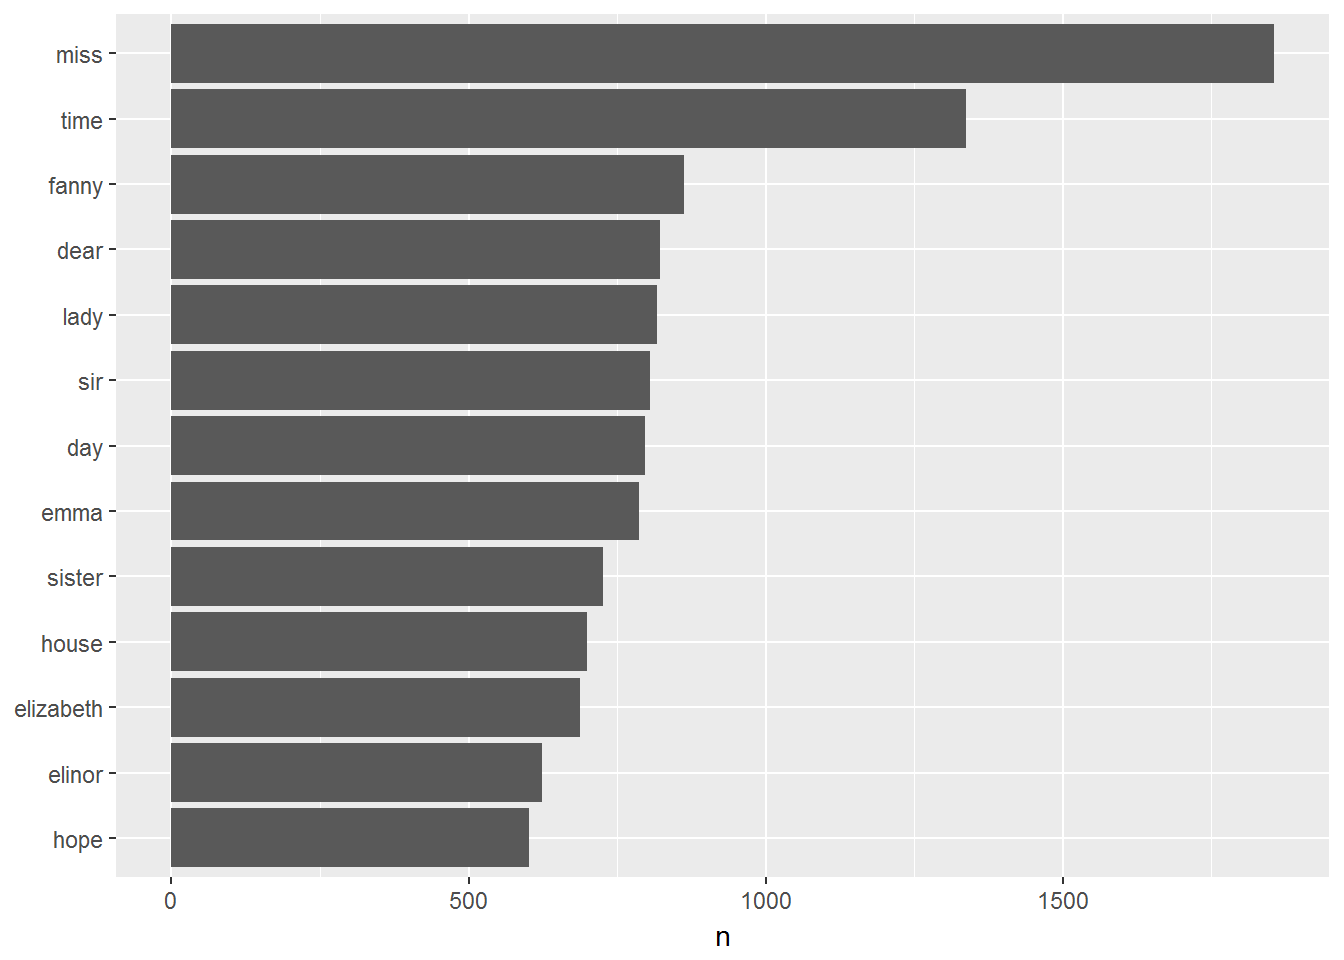
\includegraphics{IntroTextMining_files/figure-latex/unnamed-chunk-40-1.pdf}

O, mediante una nube de palabras utilizando el paquete
\texttt{wordcloud}:

\begin{Shaded}
\begin{Highlighting}[]
\KeywordTok{require}\NormalTok{(wordcloud)}
\end{Highlighting}
\end{Shaded}

\begin{verbatim}
## Warning: package 'wordcloud' was built under R version 3.4.4
\end{verbatim}

\begin{Shaded}
\begin{Highlighting}[]
\KeywordTok{wordcloud}\NormalTok{(}\DataTypeTok{words =}\NormalTok{ freq}\OperatorTok{$}\NormalTok{word, }\DataTypeTok{freq =}\NormalTok{ freq}\OperatorTok{$}\NormalTok{n, }\DataTypeTok{min.freq =} \DecValTok{300}\NormalTok{,}
          \DataTypeTok{max.words=}\DecValTok{100}\NormalTok{, }\DataTypeTok{random.order=}\OtherTok{FALSE}\NormalTok{, }\DataTypeTok{rot.per=}\FloatTok{0.35}\NormalTok{, }
          \DataTypeTok{colors=}\KeywordTok{brewer.pal}\NormalTok{(}\DecValTok{8}\NormalTok{, }\StringTok{"Dark2"}\NormalTok{))}
\end{Highlighting}
\end{Shaded}

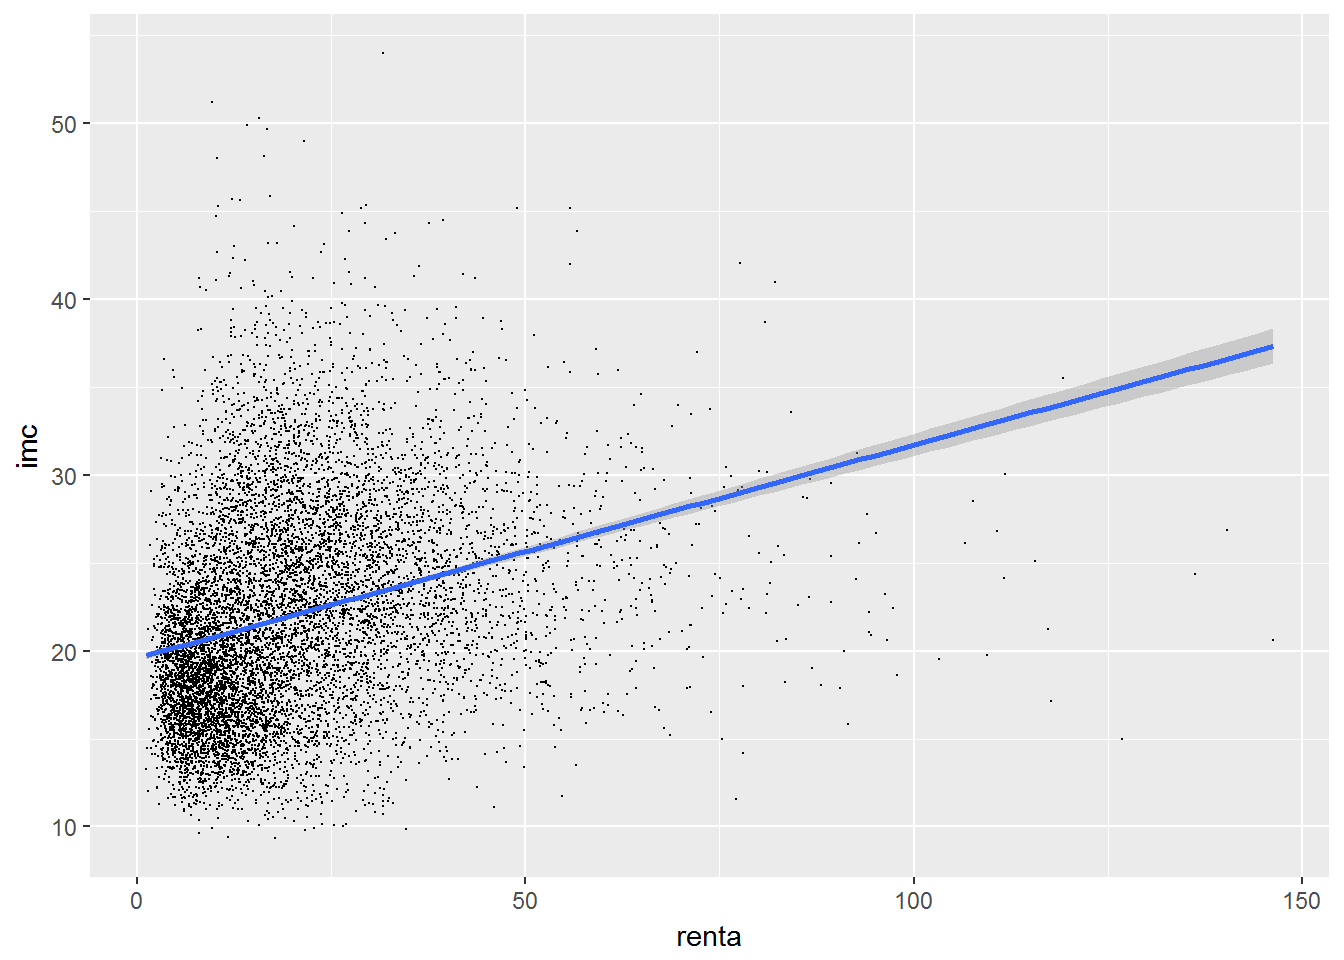
\includegraphics{IntroTextMining_files/figure-latex/unnamed-chunk-41-1.pdf}

Otro enfoque es observar la frecuencia inversa de documentos
(\texttt{idf}) para una palabra dada, que aumenta su peso si se usa en
pocos documentos de la colección:

Si \(N\) denota el número total de documentos y \(N_p\) el número de
documentos que contienen la palabra \(p\), entonces el \texttt{idf} de
dicha palabra es: \[
\mbox{idf} = - \log\left(\frac{N_p}{N}\right)
\]

Esto se puede combinar con la frecuencia de la palabra \texttt{tf} para
calcular el \texttt{tf-idf} de un término (\texttt{producto\ de\ ìdf}y
\texttt{tf}), es decir, la frecuencia de una palabra multiplicado por su
especificidad al documento.

Por lo tanto, la medida \texttt{tf-idf} mide hasta que punto una palabra
caracteriza un documento dado dentro de una colección (o corpus) al cual
pertenece dicho documento.

Si lo aplicamos a las novelas de Jane Austeen, obtenemos:

\begin{Shaded}
\begin{Highlighting}[]
\NormalTok{book_words <-}\StringTok{ }\KeywordTok{austen_books}\NormalTok{() }\OperatorTok\StringTok{ }\KeywordTok{unnest_tokens}\NormalTok{(word, text) }\OperatorTok
\StringTok{  }\KeywordTok{count}\NormalTok{(book, word, }\DataTypeTok{sort =} \OtherTok{TRUE}\NormalTok{) }\OperatorTok
\StringTok{  }\KeywordTok{ungroup}\NormalTok{()}

\NormalTok{freq_rel <-}\StringTok{ }\NormalTok{book_words }\OperatorTok\StringTok{ }\KeywordTok{bind_tf_idf}\NormalTok{(word, book, n)}
\NormalTok{freq_rel}
\end{Highlighting}
\end{Shaded}

\begin{verbatim}
## # A tibble: 40,379 x 6
##    book              word      n     tf   idf tf_idf
##    <fct>             <chr> <int>  <dbl> <dbl>  <dbl>
##  1 Mansfield Park    the    6206 0.0387    0.     0.
##  2 Mansfield Park    to     5475 0.0341    0.     0.
##  3 Mansfield Park    and    5438 0.0339    0.     0.
##  4 Emma              to     5239 0.0325    0.     0.
##  5 Emma              the    5201 0.0323    0.     0.
##  6 Emma              and    4896 0.0304    0.     0.
##  7 Mansfield Park    of     4778 0.0298    0.     0.
##  8 Pride & Prejudice the    4331 0.0354    0.     0.
##  9 Emma              of     4291 0.0267    0.     0.
## 10 Pride & Prejudice to     4162 0.0341    0.     0.
## # ... with 40,369 more rows
\end{verbatim}

Podemos observar que para estas palabras de uso muy corriente
\texttt{idf} es igual a cero. Para ver las palabras con una elevada
importancia escribimos:

\begin{Shaded}
\begin{Highlighting}[]
\NormalTok{freq_rel }\OperatorTok\StringTok{ }\KeywordTok{arrange}\NormalTok{(}\KeywordTok{desc}\NormalTok{(tf_idf))}
\end{Highlighting}
\end{Shaded}

\begin{verbatim}
## # A tibble: 40,379 x 6
##    book                word          n      tf   idf  tf_idf
##    <fct>               <chr>     <int>   <dbl> <dbl>   <dbl>
##  1 Sense & Sensibility elinor      623 0.00519  1.79 0.00931
##  2 Sense & Sensibility marianne    492 0.00410  1.79 0.00735
##  3 Mansfield Park      crawford    493 0.00307  1.79 0.00551
##  4 Pride & Prejudice   darcy       373 0.00305  1.79 0.00547
##  5 Persuasion          elliot      254 0.00304  1.79 0.00544
##  6 Emma                emma        786 0.00488  1.10 0.00536
##  7 Northanger Abbey    tilney      196 0.00252  1.79 0.00452
##  8 Emma                weston      389 0.00242  1.79 0.00433
##  9 Pride & Prejudice   bennet      294 0.00241  1.79 0.00431
## 10 Persuasion          wentworth   191 0.00228  1.79 0.00409
## # ... with 40,369 more rows
\end{verbatim}

Y así podemos representar una caracterización de cada novela mediante
dichas palabras:

\begin{Shaded}
\begin{Highlighting}[]
\NormalTok{freq_rel }\OperatorTok\StringTok{ }\KeywordTok{arrange}\NormalTok{(}\KeywordTok{desc}\NormalTok{(tf_idf)) }\OperatorTok
\StringTok{  }\KeywordTok{mutate}\NormalTok{(}\DataTypeTok{word =} \KeywordTok{factor}\NormalTok{(word, }\DataTypeTok{levels =} \KeywordTok{rev}\NormalTok{(}\KeywordTok{unique}\NormalTok{(word)))) }\OperatorTok\StringTok{ }
\StringTok{  }\KeywordTok{group_by}\NormalTok{(book) }\OperatorTok\StringTok{ }
\StringTok{  }\KeywordTok{top_n}\NormalTok{(}\DecValTok{15}\NormalTok{) }\OperatorTok\StringTok{ }
\StringTok{  }\KeywordTok{ungroup}\NormalTok{() }\OperatorTok
\StringTok{  }\KeywordTok{ggplot}\NormalTok{(}\KeywordTok{aes}\NormalTok{(word, tf_idf, }\DataTypeTok{fill =}\NormalTok{ book)) }\OperatorTok{+}
\StringTok{  }\KeywordTok{geom_col}\NormalTok{(}\DataTypeTok{show.legend =} \OtherTok{FALSE}\NormalTok{) }\OperatorTok{+}
\StringTok{  }\KeywordTok{labs}\NormalTok{(}\DataTypeTok{x =} \OtherTok{NULL}\NormalTok{, }\DataTypeTok{y =} \StringTok{"tf-idf"}\NormalTok{) }\OperatorTok{+}
\StringTok{  }\KeywordTok{facet_wrap}\NormalTok{(}\OperatorTok{~}\NormalTok{book, }\DataTypeTok{ncol =} \DecValTok{2}\NormalTok{, }\DataTypeTok{scales =} \StringTok{"free"}\NormalTok{) }\OperatorTok{+}
\StringTok{  }\KeywordTok{coord_flip}\NormalTok{()}
\end{Highlighting}
\end{Shaded}

\begin{center}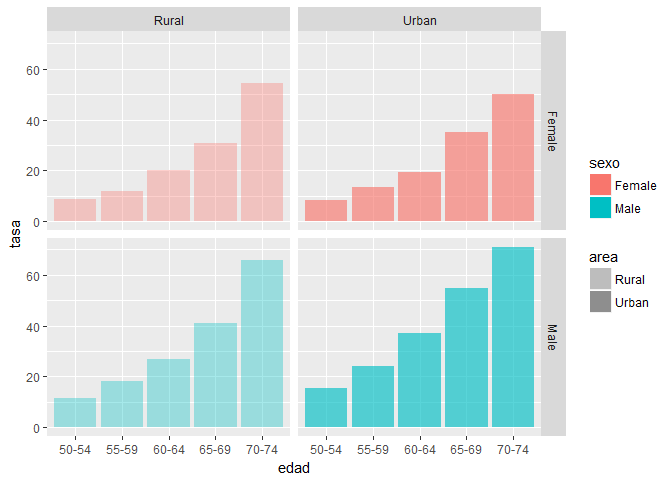
\includegraphics{IntroTextMining_files/figure-latex/unnamed-chunk-44-1} \end{center}

\begin{ej}
Caracterizar algunos capítulos de ``Pride and Prejudice'' mediante el
indicador \texttt{tf-idf}.
\end{ej}

\begin{ej}
Descargar 20 discursos del rey de España y caracterizarlos. Utilizar la
dirección siguiente donde \emph{data} corresponde al número del
discurso.

\url{http://www.casareal.es/ES/Actividades/Paginas/actividades_discursos_detalle.aspx?data=5738}
\end{ej}

\begin{nota}
De manera general, se puede importar libros mediante el
\href{!https://www.gutenberg.org/}{proyecto Gutenberg} y el paquete
\texttt{gutenbergr} (Robinson, 2016). Así, se puede importar la novela
``Niebla'' de Unamuno, de la siguiente manera:
\end{nota}

\begin{Shaded}
\begin{Highlighting}[]
\KeywordTok{require}\NormalTok{(gutenbergr)}
\NormalTok{unamuno <-}\StringTok{ }\KeywordTok{gutenberg_works}\NormalTok{(title}\OperatorTok{==}\StringTok{"Niebla}\CharTok{\textbackslash{}n}\StringTok{(Nivola)"}\NormalTok{,}\DataTypeTok{languages=}\StringTok{"es"}\NormalTok{)}\OperatorTok{$}\NormalTok{gutenberg_id }\OperatorTok
\KeywordTok{gutenberg_download}\NormalTok{() }\OperatorTok\StringTok{ }
\KeywordTok{gutenberg_strip}\NormalTok{() }\CommentTok{#quita encabezado y pie de pagina}
\end{Highlighting}
\end{Shaded}

\section{Referencias}\label{referencias}

Este curso está basado en los siguientes textos:

\begin{itemize}
\item
  \emph{R para profesionales de los datos}, Carlos Bellosta, 2017,
  \href{https://datanalytics.com/libro_r}{\texttt{https://datanalytics.com/libro\_r}}
\item
  \emph{Text Mining with R, A Tidy Approach}, Julia Silge and David
  Robinson, 2018,
  \href{https://www.tidytextmining.com/tidytext.html}{\texttt{https://www.tidytextmining.com/tidytext.html}}
\item
  \emph{Scraping HTML Text}, Bradley Boehmke, 2015,
  \href{http://bradleyboehmke.github.io/2015/12/scraping-html-text.html}{\texttt{http://bradleyboehmke.github.io/2015/12/scraping-html-text.html}}
\end{itemize}


\end{document}
